
The major contribution of this work is providing a task modeling and setup for learning humanoid  movements in the RoboCup Soccer3D domain using reinforcement learning frameworks. More specifically, we learned several variations of a kick motion, creating behaviors capable of imitating the ZMP kick, reaching a much farther position for the ball, and reaching a desired fixed final distance for the ball.


We also introduce the deep mimic approach for this class of problems and a specific curriculum to learn, as well as several implementation considerations, manually tunned and developed after a few iterations.

\section{Environment and Implementation}

As previously mentioned in Chapter \ref{chap:method}, this work used the RL algorithms implementations from the OpenAI baselines repository \cite{baselines}. More specifically, the high-quality implementation of PPO. Not implementing the DRL algorithms from scratch made it much easier to test, iterate, improve and focus on developing the agent experiments.

The PPO implementation on Baselines was adapted to change the communication with the OpenAI Gym environments to communicate with the Soccer3D agent, maintaining the same function protocols.

The framework used to integrate the baselines code with new experiments, flexible to develop, in the Soccer3D domain was already built in the work \cite{TGMuzio}. This framework can be basically described by its two main modules, each one running as a separate process and communicating through Protocol Buffers.

\begin{itemize}
\item \textbf{Learning Client:} Process that runs the reinforcement learning algorithms and makes remote procedure calls (RPCs) to the server, exchanging state/action information with the soccer agent. This module was implemented in Python 3.5 and TensorFlow, using OpenAI Baselines implementations.

\item \textbf{Soccer Agent:} The simulated agent which interacts with \textit{SimSpark} and with the learning client, executing the learning experiments. This module was implemented in C++ and uses the ITAndroids Soccer Simulation 3D code base.
\end{itemize}

As already commented, the API between server and client uses Protocol Buffers, with the exchange of RPCs containing the standard state, action, reward and end of episode information used in OpenAI Gym. An illustration of this framework follows in the diagram presented in Figure \ref{fig:RL_framework}. For details, please refer to \cite{TGMuzio}.

\begin{figure}[H]
    \centering
    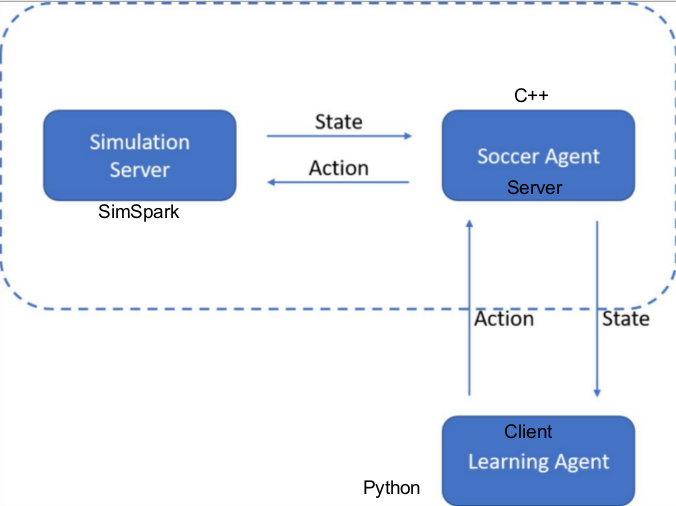
\includegraphics[width=0.8\textwidth]{Chapter6/architecture.png} 
    \caption{Learning Architecture diagram. Extracted from \cite{TGMuzio}}
    \label{fig:RL_framework}
\end{figure}

\section{Infrastructure}

This work used the Intel AI DevCloud as its main infrastructure to run all learning experiments described below.

The cluster is composed by 10 computation nodes using each one a 24 cores Intel Xeon processor. Furthermore, the experiments setup exploited the parallelization feature of PPO, running up to 12 Soccer Agents per node, besides the Learning Client process, and collecting a total number of samples in the magnitude of 100 million.

\section{Deep Mimic Learning}
\label{sec:deep_mimic}

The Deep Mimic approach \cite{deepmimic} established a great new paradigm in which this work was based on. It introduces a novel idea of allowing the supply of reference motions from motion capture or hand-authored animation data for style, and then generating goal-directed and physically realistic behavior from those reference motions \cite{deepmimic}.

The basic approach presented for this mission consists in rewarding the agent to reproduce motions that resemble the reference data, as well as to achieve additional task objectives.

In the original work, a control policy $\pi (a_t|s_t,g_t)$ maps the state of the character $s_t$ and a task-specific goal $g_t$ to an action $a_t$. The action distribution is gaussian, with fixed covariance and mean given by a neural network. This policy outputs the desired joints positions, which is later translated into torque commands by each joint PD controller.

The overall reward is splitted into the imitation reward, given by $r_I(s_t,a_t)$, and the task-specific reward, given by $r_G(s_t,a_t)$, with corresponding weights given by $\omega^I$ and $\omega^G$, respectively. The final reward is therefore given by Equation \eqref{eq:deep_mimic_reward}.

\begin{equation}
r_t = \omega^I r_t^I + \omega^G r_t^G
\label{eq:deep_mimic_reward}
\end{equation}

The policies are trained with PPO using the clipped surrogate objective, maintaining also a further network for the value function $V_{\psi}(s,g)$.

It is worth mentioning that this work introduces also two novel ideas which significantly increased the robustness and performance of the learning behaviors. 

\begin{itemize}
\item \textit{Reference State Initialization} (RSI) randomly selects a state in which the agent and its reference actor begins at each episode. In this way, it makes possible to discover high reward future states without the need to learn everything until then, which can be very significant in difficult tasks like backflips.

\item \textit{Early Termination} (ET) finishes the episode when the agent reaches any fruitless condition, such as a fall or joints collision. This process discourage undesirable behaviors and the exploration of bad states, therefore increasing the learning efficiency.
\end{itemize}

\section{Experiments}

In this section, we describe the learning experiments conducted in this work. The ultimate goal is learning a complete behavior capable of kicking the ball towards a planned final distance fed into the input of the policy, however, we started by learning simpler problems. These problems were very useful not only in providing a curriculum learning approach \cite{BengioCurrLearning} and therefore the basements to achieve the final goal, but also helping to validate all the setup, algorithms and to get a better understanding of the problem and the simulation environment limitations.

\subsection{Supervised Kick Learning}

The first trial of learning a kick behavior was basically learning to imitate the reference kick movement using supervised learning techniques. Therefore, for this experiment, there was no need to use the RL setup or to run a learning agent.

Once the reference movement is deterministic, the neural network used has only one input given by time itself. Two fully-connected hidden layers follow, composed by 512 LeakyRelu hidden units each one. Finally, we have a output layer given by 22 linear units, providing position commands for all 22 agent joints.

%For training, we used Adam optimization, applying 5 consecutive optimization cycles with 5000 epochs each one and decreasing the learning rate linearly, applying $10e^{-4}$, $8e^{-4}$, $6e^{-4}$, $4e^{-4}$, $2e^{-4}$ respectively for each cycle.

\subsection{Pure Mimic Learning}

The second checkpoint to achieve was still learning to imitate the reference movement, reaching the best possible precision. However, since we wanted also to validate and test the learning setup, we chose the reinforcement learning approach, using the Proximal Policy Optimization algorithm.

\textbf{State space:} Since the reference movement is deterministic and the commanded actions only depend of the point in time, the 1D observation space consists on the episode timestep solely, given by a multiple of the simulator unit step $0.02s$.

\textbf{Action space:} We decided to restrict the action space to the joints with biggest impact in the kick distance, in order to reduce the learning cost for this task. Therefore, the 6D action space consists on the position commands for the 6 joints of the kicking leg. These position commands are sequentially fed into PID controllers on each joint, in order to generate velocity commands to the motors, which are finally sent to Simspark. It is also worth mention that the other 16 joints will be driven by the ZMP kick engine.

\textbf{Reward signal:} The reward is given by:

\begin{equation}
r_t = -\sum_{j=1}^{6}{|q_t^j-\hat{q}_t^j|^2}
\end{equation}

Where $q_t^j$ and $\hat{q}_t^j$ represent the commanded positions to the $j$-$th$ joint at instant $t$ from the learning agent and from the reference movement, respectively. Therefore, we basically penalize the square difference of the commands given to all 6 joints.

The reference movement used was the ZMP kick, described in the previous chapter. We also used a fully-connected NN with two hidden layers, and 512 LeakyRelu units each one, followed by an output layer with 6 units.

Besides, in order to simplify the problem in a first moment, we ran everything offline, by comparing the network output with the reference data in a file, without the need to initialize the simulated agent. In this way, we can avoid the physical restrictions involved, and some limitations such as the robot falls, and therefore speeding up the learning process.

Furthermore, the biggest achievement from this task was obtaining a policy network that can also be used as the starting point for the following learning tasks. In this way, it already provides a big learning step in the process of reaching the ultimate goal.

We also conducted successful experiments which learned to imitate for all 22 joints, but we used the 6D policy in the next experiments, in order to simplify the learning process for more complex tasks.

\subsection{Farthest Final Distance Learning}
\label{sec:far_kick_description}

The following learning task consists in kicking the ball towards the longest possible distance. The purpose is testing the limits of the kick motion, and the deviation the learning process can achieve from the base movement.

We initialized the policy and value-function networks using the resulted ones from the pure mimic task. In this way, the agent already starts knowing a basic behavior for kicking. Therefore, the state and action spaces for this task is the same of the previous task, only requiring a special design for the reward signal.

The reward function was based on the Deep Mimic work \cite{deepmimic}, thus it follows the same format described in \eqref{eq:deep_mimic_reward}. The imitation component will then be given by Equation \eqref{eq:imitation_reward}, while the goal reward is described by Equation \eqref{eq:goal_reward_farthest}.

\begin{equation}
r^I_t = \omega^p r^p_t + \omega^e r^e_t + \omega^c r^c_t
\label{eq:imitation_reward}
\end{equation}

The imitation component in \eqref{eq:imitation_reward} is still composed by three other factors.

The pose reward $r^p_t$ is given by Equation \eqref{eq:position_imitation}, where $q_t^j$ and $\hat{q}_t^j$ represent the actual positions during motion of the $j$-$th$ joint at instant $t$ from the learning agent and from the reference movement, respectively, and encourages the agent to match the joint orientation of the reference motion at each step. In \eqref{eq:position_imitation} we sum up to $n$ joints, but we will actually use $n=6$, corresponding to the 6 joints of the kicking leg.

\begin{equation}
r^p_t = \exp{ \left[ -2 \left( \sum_{j=1}^{n}{|q_t^j-\hat{q}_t^j|^2} \right) \right] }
\label{eq:position_imitation}
\end{equation}

The end-effector reward $r_t^e$ is given by Equation \eqref{eq:end_effector_imitation}, where $p_t^e$ and $\hat{p}_t^e$ represent the kicking feet positions from the learning agent and reference movement, respectively, and encourages the agent feet to match the positions from the reference movement.

\begin{equation}
r^e_t = \exp{ \left[ -40 |p_t^e-\hat{p}_t^e|^2 \right]}
\label{eq:end_effector_imitation}
\end{equation}

At last for imitation, the center-of-mass reward $r_t^c$ is given by Equation \eqref{eq:CM_imitation}, and penalizes the deviation between the agent CoM $p_t^c$ and the reference CoM $\hat{p}_t^c$.

\begin{equation}
r^c_t = \exp{ \left[ -10 |p_t^c-\hat{p}_t^c|^2 \right]}
\label{eq:CM_imitation}
\end{equation}

Finally, we have the goal reward component $r_t^G$ described in Equation \eqref{eq:goal_reward_farthest}. This expression basically encourages the longest distance between ball's final and initial positions, giving a big exponential reward. It is worth to notice that this reward signal is given at each episode timestep, encouraging also the agent to kick the ball as fast as possible.

\begin{equation}
r_t^G = \exp{ \left[ 7 (\text{ballPos - ballInitPos}) \right]}
\label{eq:goal_reward_farthest}
\end{equation}

This task was very useful in obtaining a new learned behavior for the first time, starting from the mimic base behavior. Hence, it helped to discover the limitations and particularities of this challenge, improving our overall knowledge about it.

\subsection{Fixed Final Distance Learning}

The next learning task consists in kicking the ball towards a fixed final distance, hardly inputed as a constraint in the reward function.

Following the same approach described for the Farthest Final Distance task in the previous section, in this task we also started with the policy and value-function MLPs developed in the Pure Mimic task. In this sense, we maintain the same state and action space.

The reward function follows the Deep Mimic design and is composed by a imitation component and a goal oriented component, described in \eqref{eq:deep_mimic_reward}. The imitation component has the same shape presented for the Farthest Final Distance task, introduced by Equations \eqref{eq:imitation_reward}, \eqref{eq:position_imitation}, \eqref{eq:end_effector_imitation} and \eqref{eq:CM_imitation}.

The goal reward component $r^G_t$, however, introduces a new design, specifically hard coded for each fixed distance experiment.

We conducted two experiments for learning to kick the ball towards the final positions of $0.8m$ and $1.5m$, however, it could be analogously replicated for other distances within the limits of the maximum distance reached in the previous task.

The goal reward function for the fixed positions of $0.8m$ and $1.5m$ experiments are given by Equations \eqref{eq:08_fixed_reward} and \eqref{eq:15_fixed_reward}, respectively.

\begin{equation}
10^4 exp \left( -10 |\text{ballFinalPos}-0.8| \right)
\label{eq:08_fixed_reward}
\end{equation}

\begin{equation}
10^4 exp \left( -10 |\text{ballFinalPos}-1.5| \right)
\label{eq:15_fixed_reward}
\end{equation}

The idea is to provide a big encouragement for reaching a final distance close to the desired target. This reward component is usually much bigger than the imitation one, in order to allow some significant deviations from the base movement capable of making possible to reach the goal.

Different than the Farthest Final Distance task, this goal reward component is only given at the end of the episode, after the ball stops, since we wanted to encourage precision rather than speed. This approach makes the reward function very sparse, introducing some challenges in the process.

The experiments implementation details, as well as the reward weights and hyperparameters will be presented in the next chapter.






